
\chapter{2D wings in compressible flow}
\setcounter{section}{1}

\section{Transonic flows}
\subsection{Drag divergence Mach number}
	\wrapfig{22}{l}{4.5}{0.5}{ch6/1}{fig:6.1}
	At the critical Mach number $M_\infty = M_{cr}$, the flow reaches $M=1$ somewhere on the wing. If the velocity at $\infty$ is increased, $M_\infty$ also (still <0), a small area where the flow becomes \textbf{supersonic} will develop on the \textbf{suction side}. For increasing $M_\infty$ this area will growth and at a certain $M_\infty$ a \textbf{shock wave} will develop, as a result of which the flow will become \textbf{subsonic} again (the supersonic area abruptly terminated). Such area also develops on the \textbf{pressure side} at high $M_\infty$ (\autoref{fig:6.1} (a)).
	
	\ \\ If $M_\infty$ increases further, the supersonic regions further extends and the shock waves moves downstream, the one on the pressure side more rapidly (\autoref{fig:6.1} (b) (c)). As soon as the shock waves are strong enough, they can cause separation of the boundary layer, this separation is the \textbf{shock stall} and the $M_\infty$ where this happen is called the \textbf{drag divergence Mach number}. Indeed, the drag suddenly increases as result of the separation, this called \textbf{transonic drag rise}, shown on \autoref{fig:6.2}. 
	
	\ \\ For further increase of $M_\infty <1$, the shock wave on the pressure side eventually reaches the trailing edge (\autoref{fig:6.1} (d)). In a certain Mach number range, the shock wave manifests the so-called $\bm{\lambda}$ \textbf{shocks}. Near the profile the shock has two legs, a first oblique one through which the flow is slowed down but remains supersonic, and a second normal one through which the flow becomes subsonic. 
	
	\ \\ Eventually the shock wave on the suction side can also reach the trailing edge and give birth to the \textbf{bifurcated trailing edge shock} patern (\autoref{fig:6.1} (e)). 
	
	\ \\ For further increase of $M_\infty$ there is no change, till $M_\infty$ exceeds 1. In this case, a so-called \textbf{detached bow shock} develops upstream of the leading edge. There is a small subsonic region between this shock and the leading edge. This manifests both for thick, bounded leading edge and thin one (\autoref{fig:6.1} (f) (g)). In the second case, the bow shock changes into 2 oblique shocks at the leading edge for increasing $M_\infty$ (\autoref{fig:6.1} (h)). This happens at the \textbf{shock attachment Mach number}, $\bm{M_{SA}}$. For further $M_{\infty}$, the flow becomes fully supersonic and the drag decreases. In the case of rounded leading edge, the bow shock continues to exist and comes closer to the leading edge. 
	
	\begin{center}
	\begin{minipage}{0.3\textwidth}
	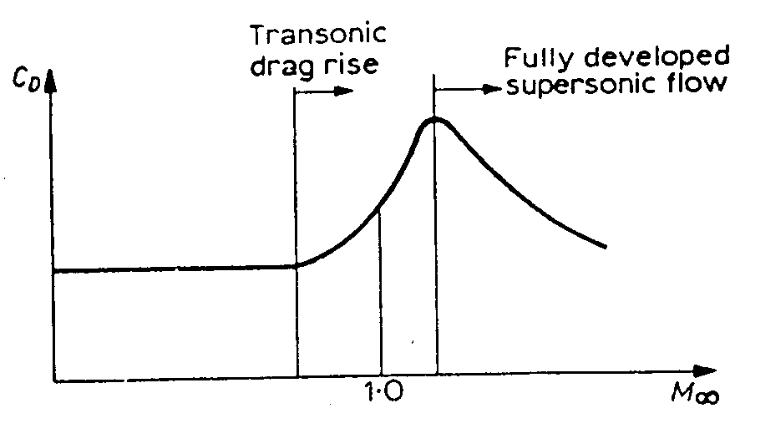
\includegraphics[scale=0.3]{ch6/2}
	\captionof{figure}{}
	\label{fig:6.2}
	\end{minipage}
	\begin{minipage}{0.3\textwidth}
	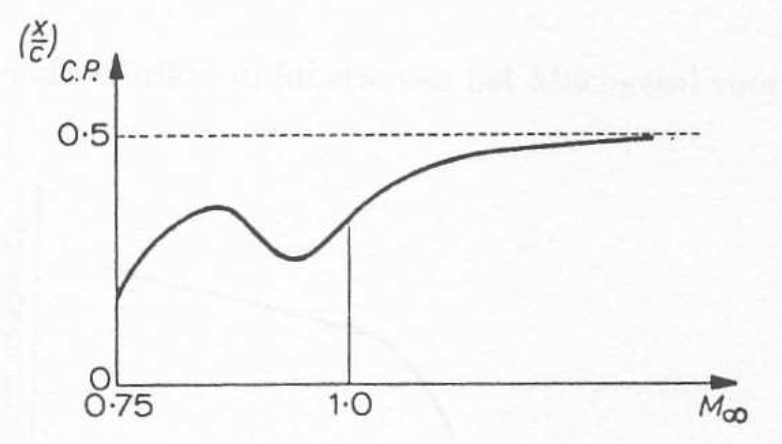
\includegraphics[scale=0.3]{ch6/3}
	\captionof{figure}{}
	\label{fig:6.3}
	\end{minipage}
	\end{center}
	
	Under transonic conditions the flow is non-stationary, the shock waves moves up and down on the wing. The pilot senses this as \textbf{buffeting} (response of the structure to aerodynamic excitation) and vibrations. This can make the plane uncontrollable or cause serious damages. The cause of the excitation is the fluctuating pressure in non-stationary conditions. Normally one flies under the buffeting margin but one can exceed it in case of sudden maneuvers for fighters for example. \\
	
	The center of pressure is also moving with $M_\infty$ (\autoref{fig:6.3}). First, it goes backward as the shock wave going backward on the suction side makes the underpressure greater. Then, it goes forward because the shock wave on the pressure side is moving faster. The latter reaches the trailing edge while the shock wave on the suction side still moves backward, making the center of pressure again move backward, tending to the 50\% chord. This makes the control of the plane more difficult. \\
	
	\wrapfig{7}{l}{5.5}{0.3}{ch6/4}{fig:6.4}
	It is this buffeting effect that imposes an upper limit to the velocity of subsonic planes. With the increase of the drag due to separation when shock waves (shock-stall) is associated a decrease of the lift. We can see that the lift temporary increases after the lower shock reaches the trailing edge. This is explained by the smaller separation when in this location. The drag divergence Mach number is 5-10\% larger than $M_{cr}$. 
	
	\ \\
	
	\begin{center}
	\begin{minipage}{0.4\textwidth}
	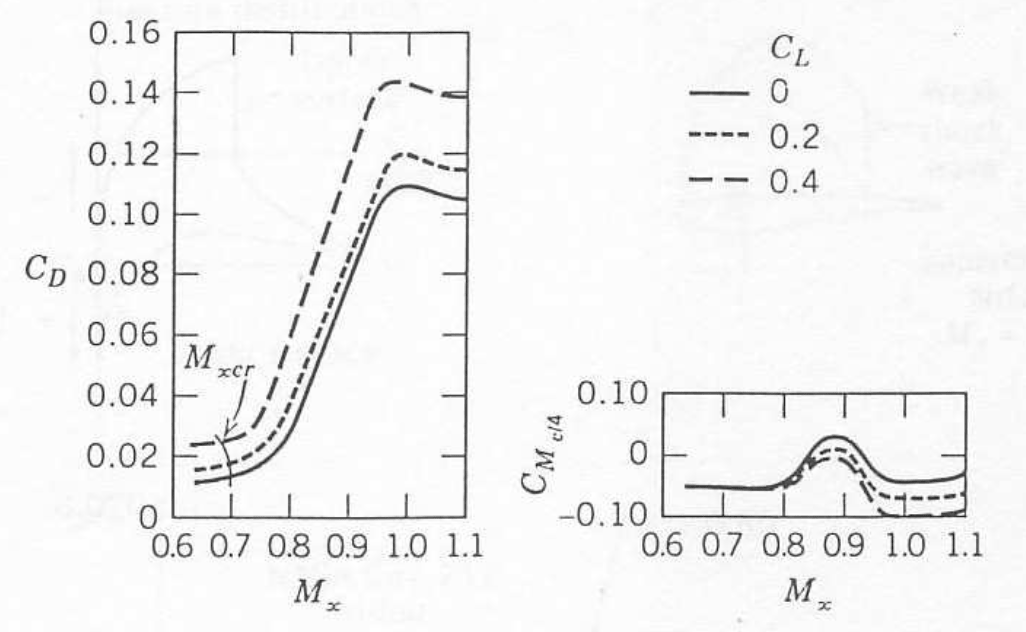
\includegraphics[scale=0.3]{ch6/5}
	\captionof{figure}{}
	\label{fig:6.5}
	\end{minipage}
	\begin{minipage}{0.4\textwidth}
	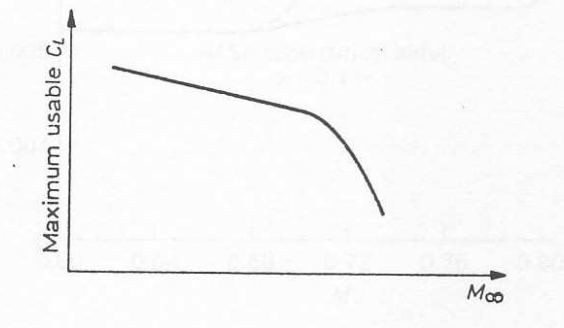
\includegraphics[scale=0.6]{ch6/6}
	\captionof{figure}{}
	\label{fig:6.6}
	\end{minipage}
	\end{center}

	On \autoref{fig:6.5} we can see the influence of increasing lift (increasing $\alpha$). We can notice that with increasing lift, the drag increases for all Mach numbers, the moment increases in the transonic region and $M_{cr}$ decreases. On \autoref{fig:6.6}, we notice that the lift coefficient strongly decreases in the transonic region due to buffering effects. 
	
\subsection{Supercritical wings}
	\wrapfig{16}{l}{9.5}{0.3}{ch6/7}{fig:6.7}
	For subsonic wings, it is thus desired to have the largest drag divergence Mach number possible. This can be achieved by using high critical Mach number wings, or increase the difference  $M_{div} -M_{cr}$. The second solution led to the supercritical wings. These have a rather flat suction side to limit the acceleration of the flow, keeping the supersonic speeds lower than other profiles and limit the strength of the shock that creates less drag. The comparison between the two type of wings is done on \autoref{fig:6.7}. We can see that the $M_{cr}$ is higher and the weaker shock wave closer to the trailing edge. 
	
	\ \\ The new shape of the suction side has a negative effect on the lift, this is compensate by an increased curvature on the pressure side near the trailing edge. On the figure we can see that the use of critical wings increases the drag divergence Mach number, that can go up to 0.99. These allows the use of thicker wings, allowing more fuel storage at lower speeds. 
	
\section{Supersonic flows}
	\subsection{The drag coefficient in a linearized supersonic flow}
	The potential equation we used in the framework of potential equation can be rewritten in the case of supersonic flow as:
	
	\begin{equation}
		(1-M_\infty^2) \hat{\phi}_{xx} + \hat{\phi}_{yy} = 0 \qquad \Rightarrow \lambda ^2 \hat{\phi} _{xx} - \hat{\phi} _{yy} = 0.
	\end{equation}
	
	The linearized potential equation corresponds to the wave equation with $\lambda ^2 = M_\infty ^2 -1 >0$. We can show that the solution of this equation is 
	
	\begin{equation}
	\hat{\phi}(x,y)= f(x\lambda y) = \hat{\phi} _{1}(x-\lambda y) + \hat{\phi} _{2} (x+\lambda y).
	\end{equation}		
	
	Let's define 2 families of characteristic curves:
	
	\begin{equation}
	\left\{
	\begin{aligned}
	&C^+ : x-\lambda y = cst \qquad \Rightarrow y = \frac{1}{\lambda} x + cst = \frac{1}{\sqrt{M_\infty ^2 -1}} c + cst\\
	&C^+ : x+\lambda y = cst \qquad \Rightarrow y = -\frac{1}{\lambda} x + cst = -\frac{1}{\sqrt{M_\infty ^2 -1}} c + cst
	\end{aligned}
	\right.
	\end{equation}
	
	\wrapfig{8}{r}{5}{0.3}{ch6/8}{fig:6.8}
	In this way, $\hat{\phi} _1$ and $\hat{\phi} _2$ are respectively constant on $C^+$ and $C^-$. The slope is denoted $\mu _\infty ^\pm$ for $C^\pm$ such that: 
	
	\begin{equation}
	\tan \mu _\infty ^\pm = \pm \frac{1}{\sqrt{M_\infty ^2 -1}} \qquad \sin \mu _\infty ^\pm = \pm \frac{1}{M_\infty}.
	\end{equation}
	
	To find the general solution in P, let's first consider the initial data given on the y-axis: 
	
	\begin{equation}
	\hat{\phi} _1(y) = F(y)\qquad \hat{\phi}_2 (y) = G(y)
	\end{equation}
	
	Now let's construc $C^+$ and $C^-$ throw P: 
	
	\begin{equation}
	C^+ : x-\lambda y = x_A - \lambda y_A\qquad C^- : x-\lambda y = x_B + \lambda y_B.
	\end{equation}
	
	Finally, the solution in P is so given by:
	
	\begin{equation}
	\hat{ \phi} (x_p,y_p) = \hat{\phi} (x_A - \lambda y_A) + \hat{\phi} _2 (x_B + \lambda y_B) = F (x_A - \lambda y_A) + G (x_B + \lambda y_B)
	\end{equation}
	
\subsubsection{Application to a flat plate}
	